\documentclass[10pt]{book}
\usepackage[top=2cm, bottom=1.5cm, left=2.5cm, right=2.5cm]{geometry}
\usepackage{graphicx} % Required for inserting images
\usepackage{algorithm} % algorithm block
\usepackage{algpseudocode}
\algrenewcommand\algorithmicrequire{\textbf{Input:}} % change REQUIRE to Input
\algrenewcommand\algorithmicensure{\textbf{Output:}}

\usepackage{booktabs} %pandas to latex
\usepackage{graphicx} %\resizebox

\usepackage[dvipsnames]{xcolor}
\usepackage{amsmath}
\usepackage{amssymb}
\usepackage{amsthm} % proof section
\usepackage{indentfirst}  %indent in the first line
\setlength{\parindent}{2em}

\usepackage{algorithm}
\usepackage{algorithmicx}
\usepackage{algpseudocode}
\renewcommand{\algorithmicrequire}{\textbf{Input:}} % Use Input in the format of Algorithm
\renewcommand{\algorithmicensure}{\textbf{Output:}} % Use Output in the format of Algorithm
\algnewcommand{\algorithmicand}{\textbf{and }}
\algnewcommand{\algorithmicor}{\textbf{or }}
\algnewcommand{\OR}{\algorithmicor}
\algnewcommand{\AND}{\algorithmicand}
\makeatletter
\newenvironment{breakablealgorithm}
  {% \begin{breakablealgorithm}
  \begin{center}
     \refstepcounter{algorithm}% New algorithm
     \hrule height.8pt depth0pt \kern2pt% \@fs@pre for \@fs@ruled
     \renewcommand{\caption}[2][\relax]{% Make a new \caption
      {\raggedright\textbf{\ALG@name~\thealgorithm} ##2\par}%
      \ifx\relax##1\relax % #1 is \relax
         \addcontentsline{loa}{algorithm}{\protect\numberline{\thealgorithm}##2}%
      \else % #1 is not \relax
         \addcontentsline{loa}{algorithm}{\protect\numberline{\thealgorithm}##1}%
      \fi
      \kern2pt\hrule\kern2pt
     }
  }{% \end{breakablealgorithm}
     \kern2pt\hrule\relax% \@fs@post for \@fs@ruled
  \end{center}
  }

\usepackage{mathrsfs} %for \mathscr

\usepackage{parskip} % paraskip

\usepackage[colorlinks=true,linkcolor=blue,citecolor=red,urlcolor=magenta]{hyperref}  % hyperlink

\newtheorem{thm}{Theorem}[section]
\newtheorem{pp}{Principle}[section]
\newtheorem{lem}{Lemma}[section]
\newtheorem{cor}{Corollary}[section]
\newtheorem{defn}{Definition}[section]
\newtheorem{rmk}{Remark}[section]

% proof
\newcommand{\pf}[2]{\begin{proof}[Proof for Theorem~#1]#2\end{proof}}
\newcommand{\pfsk}[2]{\begin{proof}[Proof sketch for Theorem~#1]#2\end{proof}}
\newcommand{\pfm}[3]{\begin{proof}[Proof for #1~#2]#3\end{proof}}
\newcommand{\pfskm}[3]{\begin{proof}[Proof sketch for #1~#2]#3\end{proof}}

% thm enviroment with feastures
\usepackage{tcolorbox}
% \newenvironment{blackboxtheorem}[1][]{\begin{tcolorbox}[colback=white,colframe=black,title=Problem:~#1]}{\end{tcolorbox}} % generate a blackbox environment
\newtcolorbox{problembox}[1][]{}  % generate a problem section with black box
\newtheorem{prob}{Problem}[section] % Define prob with section number
\numberwithin{prob}{section} % Number problems within sections
\tcolorboxenvironment{prob}{colback=white,colframe=black,fonttitle=\bfseries}


\newcommand{\PP}{\mathbb{P}}
\newcommand{\E}{\mathbb{E}}
\newcommand{\R}{\mathbb{R}}
\newcommand{\fnorm}[1]{\|#1\|_F}
\newcommand{\snorm}[1]{\|#1\|}
\newcommand{\xb}[1]{\textcolor{OliveGreen}{xiaobo: #1}}
\newcommand{\addtba}{\tba{(tba)}}
\newcommand{\mc}[1]{\mathcal{#1}}
\newcommand{\mb}[1]{\mathbb{#1}}
\newcommand{\mf}[1]{\mathbf{#1}}
\newcommand{\rn}[1]{\R^{#1\times #1}}
\newcommand{\rnm}[2]{\R^{#1\times #2}}
\newcommand{\td}[1]{\tilde{#1}}
\newcommand{\wtd}[1]{\widetilde{#1}}
\newcommand{\pmn}[1]{\{\pm1\}^{#1}}


% big brackets
\newcommand{\bbr}[1]{\left(#1\right)}
\newcommand{\bbfr}[1]{\left[#1\right]}
\newcommand{\bbwr}[1]{\left\{#1\right\}}

% statistics
\newcommand{\indep}{\perp \!\!\! \perp}

% \usepackage{biblatex} %Imports biblatex package
% \addbibresource{cite.bib} %Import the bibliography file
\usepackage{cite}

\title{Informational-computational trade-off in randomized numerical linear algebra}
\author{Xiaobo Yang}
\date{April 2023}

\begin{document}

\allowdisplaybreaks % allow align* enviroment cross pages

\setlength{\parindent}{2em}

\maketitle

\tableofcontents\newpage
%---------------------------------------------------
%---------------------------------------------------
%---------------------------------------------------
\chapter*{Preface}
Explore information-theoretic lower bound and computational threshold(an upper bound yielded by algorithm) in randomized numerical linear algebra. We hope the gap is as small as possible.
%---------------------------------------------------
%---------------------------------------------------
%---------------------------------------------------

\chapter{Practical Applications}
Some coding and practical projects.
%---------------------------------------------------
%---------------------------------------------------
\section{Datasets}
\xb{wiki,arxiv matrix\cite{mmmw21}}


%---------------------------------------------------
%---------------------------------------------------
\section{Statistical applications}

%---------------------------------------------------
\subsection{Gaussian process}
\xb{train gaussian process in \cite{jpwz21}\cite{mmmw21}}

%---------------------------------------------------
%---------------------------------------------------
%---------------------------------------------------
\chapter{Theory for application}
Specific complexity theory of specific applications in some areas.

%---------------------------------------------------
%---------------------------------------------------
\section{Matrix-vector multiplication queries}
%---------------------------------------------------
\subsection{Low rank approximation}
\cite{bakshi2022lowrank}

\xb{reduced to estimation of minimum eigenvalue\cite{braverman2021gradient}}


%---------------------------------------------------
\subsection{Solve linear system}
\cite{braverman2021gradient}

\xb{reduced to estimation of minimum eigenvalue\cite{braverman2021gradient}}

%---------------------------------------------------
%---------------------------------------------------
%---------------------------------------------------
\chapter{Theory for areas}
General complexity theory of specific areas of problems. 

%---------------------------------------------------
%---------------------------------------------------
\section{Matrix-vector multiplication queries}
We interact with the algorithm only through inputting query vectors and outputting matrix-vector product oracles. 

%---------------------------------------------------
\subsection{Trace estimation}
\begin{prob}[trace estimation\cite{mmmw21}]
\label{tr_est}
Given a matrix $A$, we input query vectors $r_1,...,r_m$ and output product $Ar_1,...Ar_m$ to estimate $tr(A)$. 
\end{prob}


There are a two types of query vectors.
\begin{enumerate}
    \item (Adaptive) Vectors $r_1,...,r_m$ are chosen adaptively. For example, $r_2=Ar_1$. In this case, $A$ may be used for several times.
    \item (Non-adaptive) Vectors $r_1,...,r_m$ are chosen independently. In this case, $A$ can be used for only once, for example, streaming data.
\end{enumerate}

\begin{thm}[Lower bound of adaptive queries\cite{mmmw21}]
\label{tr_est_ada}
    Let $A$ be a PSD matrix. If $r_1,...,r_m$ are adaptive and with integer entries in $\{-2^b,...,2^b\}$, then we need at least $m=\Omega\bbr{\frac{1}{\epsilon(b+\log(1/\epsilon))}}$ queries to output an estimate $t$ so that, with probability at least $2/3$, $(1-\epsilon)tr(A)\le t\le (1+\epsilon)tr(A)$.
\end{thm}
\pfsk{\ref{tr_est_ada}}{
First, reduce the problem to Gap-hamming distance problem(GHD) \ref{ghd}. For any vector $s,t\in\mb R^n$, reshape $s,t$ to matrix $S,T\in\R^{n\times n}$. Let $Z=S+T$, $A=Z^TZ$. 

Then, if we estimate $tr(A)$ with error $\epsilon=1/\sqrt{n}$, we have
\begin{align*}
    &\widehat{tr(A)}\ge2(n+\sqrt{n})(1-1/\sqrt n)=2n-2 ~~~if~~\langle s,t\rangle\ge\sqrt n,\\
    &\widehat{tr(A)}\le2(n-\sqrt{n})(1+1/\sqrt n)=2n-2 ~~~if~~\langle s,t\rangle\le-\sqrt n,
\end{align*}
which means we can solve GHD problem by simply compare $\widehat{tr(A)}$ with $2n-2$.

Finally, use lower bound of GHD. The reduction above cost $O(m\sqrt{n}(\log n + b))=\Omega(n)$ bits by Theorem \ref{ghd_lower_bound}, thus we have $m=\Omega\bbr{\frac{1}{\epsilon(b+\log(1/\epsilon))}}$.
}

\begin{thm}[Lower bound of non-adaptive queries\cite{mmmw21}]
\label{tr_est_nada}
    Let $A$ be a PSD matrix. If $r_1,...,r_m$ are non-adaptive, then we need at least $m=\Omega\bbr{\frac{1}{\epsilon}}$ queries to output an estimate $t$ so that, with probability at least $3/4$, $(1-\epsilon)tr(A)\le t\le (1+\epsilon)tr(A)$.
\end{thm}
\pfsk{\ref{tr_est_nada}}{
First, solving the problem implicitly solves a testing problem with $m$ matrix-vector product oracles. 
\begin{prob}[\cite{mmmw21}]
\label{tr_est_nada_med}
    Fix $d,n\in\mb N$ such that $d\ge n$ and $n=1/\epsilon$ for $\epsilon\in(0,1]$. Let $A=G^TDG\in\R^{d\times d}$, where $G\in\R^{n\times d}$ generated by $i.i.d$ $\mc N(0,1)$ and $D=I_n:=D_1$ or $\begin{bmatrix} I_{n-1} & 0 \\ 0 & 0 \\ \end{bmatrix}:=D_2$. Consider any algorithm taking a query matrix $U\in\R^{d\times m}$ as input and outputting product oracle $AU\in\R^{d\times m}$ to identify $D$.
\end{prob}
By concentration inequality \ref{hutchinson_bound} of Hutchinson's estimator, we have that with probability at least $11/12$,
\begin{align*}
    \frac{1}{d}tr(G^TD_1 G)\ge (1-\epsilon/4)tr(D_1) ~~~and ~~~ \frac{1}{d}tr(G^TD_2 G)\le (1+\epsilon/4)tr(D_2).
\end{align*}
Then, if we estimate $t\approx tr(A)$ with probability at least $3/4$ and error $\epsilon/4$, we have
\begin{align*}
    & t\ge (1-\epsilon/4)tr(A)\ge (1-\epsilon/4)^2 d/\epsilon\ge(1-\epsilon/2)d/\epsilon ~~if~D=D_1,\\
    & t\le (1+\epsilon/4)tr(A)\le (1+\epsilon/4)^2 (1-\epsilon) d/\epsilon\le(1-\epsilon/2)d/\epsilon ~~if~D=D_2,
\end{align*}
which means we can identify $D$ by simply compare $t$ with $(1-\epsilon/2)d/\epsilon$. By union bound, the probability is at least $2/3$.


Then, this problem can be further reduced to problem \ref{spiked_wishart}. Let $M=\begin{bmatrix}N^TN \\ L^T N\end{bmatrix}$, where $N\indep L$ and $L\in\R^{n\times(d-m)}$ with $i.i.d$ $N(0,1)$. Then we have $M\stackrel{\mathrm{dist}}{=} G^TDGE_m$, where $E_m=[e_1,...,e_m]$ is the first $m$ standard basis vectors. Therefore, it suffices to run algorithm above and if the output $D=D_1$ we claim $C=I$ otherwise $C=I-zz^T$.

% By rotational invaricance of standard Gaussian vectors, WLOG $U=E_m=[e_1,...,e_m]$, the first $m$ standard basis vectors.

% For any uniformly random unit vector $z\in\R^n$, extend it to a uniformly random orthogonal matrix $Z\in\R^{n\times n}$. Let $T=ZDS$ with $S\in\R^{n\times m}$ be $i.i.d$ $\mc N(0,1)$. Then $N \stackrel{\mathrm{dist}}{=} T$ with $D=D_1$ or $D_2$. 
% Thus $N^TN\stackrel{\mathrm{dist}}{=} S^TDZ^TZDS= G_m^T D G_m$. Let $L\in\R^{n\times(d-m}$



Finally, use lower bound theorem \ref{spiked_whishart_lower_bound}, we have $m=\Omega\bbr{\frac{1}{\epsilon}}$.
}

\begin{rmk}
\begin{enumerate}
    \item Lower bound of adaptive case is smaller than non-adaptive case. It make senses since adaptive queries contain more information on $A$.
    \item The difference of two bounds is mathematically because intermediate problem \ref{tr_est_nada_med} requires oracles(columns of $U$) are non-adaptive. But GHD problem doesn't have any requirement on relationships between oracle $r$ s.
    \item This inspires us, to reduce a problem to get a lower bound, we must keep key structures of problems as many as possible. 
    
    For instance, although we can reduce the non-adaptive scenario to GHD, the resulting bound is significantly weaker. This is because we abandon the critical constraint of exclusively using independent oracles $r$ s to tackle the problem, which renders it more challenging.
\end{enumerate}
\end{rmk}

\xb{\begin{enumerate}
    \item check why are lower bounds only suitable for PSD matrix.
\end{enumerate}}

Later, \cite{jpwz21} improve the lower bound with error probability $\delta$.
\begin{thm}[Lower bound of non-adaptive queries with $\delta$-error\cite{jpwz21}]
\label{tr_est_nada_improve}
Let $A$ be a PSD matrix. If $r_1,...,r_m$ are non-adaptive, then we need at least $m=\Omega\bbr{\frac{\sqrt{\log(1/\delta)}}{\epsilon}+\frac{\log(1/\delta)}{\log\log(1/\delta)}}$ queries to output an estimate $t$ so that, with probability at least $1-\delta$, $(1-\epsilon)tr(A)\le t\le (1+\epsilon)tr(A)$.
\end{thm}
\pfsk{\ref{tr_est_nada_improve}}{
The proof is divided into two parts according to whether $\epsilon$ is small or large.

\noindent First, for small $\epsilon=O(1/\sqrt{\log(1/\delta)})$ we have $m=\Omega\bbr{\frac{\sqrt{\log(1/\delta)}}{\epsilon}}$:
\begin{enumerate}
    \item Use Yao's principle(theorem \ref{yaoprin}) we only need to find a hard distribution. Since the bound is required to satisfied by any size $n$ of matrix $A\in\R^{n\times n}$, we consider large $n$. Use theorem \ref{block_conditional} to quantify the remaining randomness after we take several matrix-vector product oracles, we can observe if the number of queries is not so large, then the remaining randomness will yield large variance and thus large error probability. 
    \item Specifically, let $W=I_n+\frac{1}{2C\sqrt{n}}(G+G^T)$ where entries of $G$ are $i.i.d.$ $\mc N(0,1)$. Then, $W$ is PSD by theorem \ref{rmt_smax_concen} and $tr(W)\le 2n$ $w.h.p.$ for large $n$, since $tr(G)\sim\mc N(0,n)$. Quantitatively, for any $\delta\in(0,1)$, take $n=\Omega(\log(1/\delta))$ then $tr(W)\le 2n$ with probability at least $1-\delta/10$. Then, for any $\epsilon=O(\frac{\sqrt{\log(1/\delta)}}{n})=O(1/\sqrt{\log(1/\delta)})$, if we just take $m=n/2=O\bbr{\frac{\sqrt{\log(1/\delta)}}{\epsilon}}$, use theorem \ref{block_conditional} we prove the best estimation precision any algorithm can achieve $w.h.p.$ is at most $c\sqrt{\log(1/\delta)}$ for $c=\Omega(1)$, which is large than required precision $\epsilon$ and thus yield lower bound $m=\Omega\bbr{\frac{\sqrt{\log(1/\delta)}}{\epsilon}}$.
\end{enumerate}

\noindent Then, for any $\epsilon\in(0,1)$, we have uniformly lower bound $m=\Omega\bbr{\frac{\log(1/\delta)}{\log\log(1/\delta)}}$:
\begin{enumerate}
    \item The problem is further reduced to a testing problem \ref{hard_psd_testing}.
    The reduction is naturally to consider trace estimation of a random matrix $B$ generated from $P$ or $Q$ and find a gap between both confidence intervals. Actually, by concentration theorem \ref{rmt_smax_concen} we have $W + 6\sqrt{\log(1/\delta)}I_n$ is PSD $w.h.p.$, and $|tr(W)|\le 2\sqrt{2}\log(1/\delta)$ since $tr(W)\sim\mc N(0,4\log(1/\delta))$. Then, for any non-adaptive trace estimation algorithm with precision $\epsilon$, consider constant $C>\frac{10(1+\epsilon)}{1-\epsilon}-6$, then for trace estimation $t$, we have
    \begin{itemize}
        \item if $B\sim P$, then $t\ge(1-\epsilon)tr(B)=(1-\epsilon)((C+6)\log^{3/2}(1/\delta)-2\sqrt{2}\log(1/\delta))>6(1+\epsilon)\log^{3/2}(1/\delta)$ with probability at least $1-2\delta$,
        \item if $B\sim Q$, then $t\le(1+\epsilon)tr(B)\le(1+\epsilon)(6\log^{3/2}(1/\delta)+2\sqrt{2}\log(1/\delta))<6(1+\epsilon)\log^{3/2}(1/\delta)$ with probability at least $1-2\delta$,
    \end{itemize}
    which distinguishes $P$ and $Q$.
    
    \item Use hardness theorem \ref{hard_psd_testing_bound} we require at least $m=\Omega\bbr{\frac{\log(1/\delta)}{\log\log(1/\delta)}}$ queries. 
\end{enumerate}

\noindent Finally, combining these two bound by simple summation, we have our final lower bound.
}

\begin{rmk}
    Add spiked component $C\log^{3/2}(1/\delta)$ in the testing problem may be a standardized trick to analyze information-theoretic lower bound. Tuning the magnitude of the spiked component, we can show the phase transition by information-theoretic toolkit.
\end{rmk}

In this problem, the gap between informational and computational threshold is small(nearly matching).

\bigskip
\begin{breakablealgorithm}
\caption{Hutch++: randomized trace estimation with \textbf{adaptive} matrix-vector queries}
\label{hutch}
\begin{algorithmic}[1]
\Require{Matrix-vector product oracle for PSD matrix $A\in\rn n$. Number $m$ of queries.}
\Ensure{Approximation to $tr(A)$.}
\State Sample $S\in\rnm n{m/3},G\in\rnm n{m/3}$ with $i.i.d.$ $\mc N(0,1)$ entries.
\State Compute an orthonormal basis $Q\in\rnm n{m/3}$ for the span of $AS$ via $QR$ decomposition.
\State \textbf{return} $t=tr(Q^TAQ)+\frac{3}{m}tr(G^T(I-QQ^T)A(I-QQ^T)G)$.
\end{algorithmic}
\end{breakablealgorithm}
\bigskip

\begin{thm}[Upper bound of adaptive queries\cite{mmmw21}]
\label{tr_est_ada_alg}
Let $m=O\bbr{\frac{\sqrt{\log(1/\delta)}}{\epsilon}+\log(1/\delta)}$. Then with probability at least $1-\delta$, Hutch++ yields an estimation $t$ such that $(1-\epsilon)tr(A)\le t \le (1+\epsilon)tr(A)$.
\end{thm}
\pfsk{\ref{tr_est_ada_alg}}{
First, 
}

\bigskip
\begin{breakablealgorithm}
\caption{NA-Hutch++: randomized trace estimation with \textbf{non-adaptive} matrix-vector queries}
\label{na_hutch}
\begin{algorithmic}[1]
\Require{Matrix-vector product oracle for PSD matrix $A\in\rn n$. Number $m$ of queries.}
\Ensure{Approximation to $tr(A)$.}
\State Fix constants $c_1,c_2,c_3$ such that $c_1<c_2$ and $c_1+c_2+c_3=1$.
\State Sample $S\in\rnm n{c_1m},R\in\rnm n{c_2m},G\in\rnm n{c_3m}$ with $i.i.d.$ $\mc N(0,1)$ entries.
\State Let $Z=AR,W=AS$
\State \textbf{return} $t=tr((S^TZ)^+(W^TZ))+\frac{1}{c_3m}(tr(G^TAG)-tr(G^TZ(S^TZ)^+W^TG))$.
\end{algorithmic}
\end{breakablealgorithm}
\bigskip

\begin{thm}[Upper bound of non-adaptive queries\cite{jpwz21}]
\label{tr_est_nada_alg}
Let $m=O\bbr{\frac{\sqrt{\log(1/\delta)}}{\epsilon}+\log(1/\delta)}$. Then with probability at least $1-\delta$, NA-Hutch++ yields an estimation $t$ such that $(1-\epsilon)tr(A)\le t \le (1+\epsilon)tr(A)$.
\end{thm}
\pfsk{\ref{tr_est_nada_alg}}{

}

%---------------------------------------------------
\subsection{Eigenvalue estimation}
\cite{braverman2021gradient}


%---------------------------------------------------
%---------------------------------------------------
%---------------------------------------------------
\chapter{Theoretic Frameworks}
General complexity frameworks for general theoretic areas.


%---------------------------------------------------
%---------------------------------------------------
\section{Meta-complexity}
Some classical problems that are usually reduced to.
%---------------------------------------------------
\subsection{Gap-hamming distance}
\begin{prob}[Gap-Hamming\cite{mmmw21}]
\label{ghd}
     Let Alice and Bob be communicating parties who hold vectors $s\in\{\pm1\}^n$ and $t\in\{\pm1\}^n$, respectively. The Gap-Hamming problem asks Alice and Bob to return
     \begin{align*}
         1~if~\langle s,t \rangle\ge \sqrt{n}~~~~~~and~~~~~~-1~if~\langle s,t \rangle\le -\sqrt{n}.
     \end{align*}
\end{prob}



In general, we need to compute the function $f(x,y)$ for $x\in \mc X, y\in\mc Y$, where $\mc X$ and $\mc Y$ are separate sources and we cannot simultaneously obtain both $x$ and $y$. Instead, we repeatedly communicate information from $x$ to $y$ or from $y$ to $x$, accumulating intermediate information during this process. Finally, we use this accumulative intermediate information to compute $f(x,y)$. The goal is to minimize the number of times of communication or the total amount of communication bits.

To formalize this communication process, a binary tree structure called a "protocol tree" $T$(Fig.\ref{proto_tree}) is used. Each possible value of $f(x,y)$ corresponds to a leaf node $L$ in $T$. The communication complexity is measured by the height $H(T)$ of the tree $T$. Notably, for any node $N$ in $T$, the set $R(N):={(x,y):(x,y)\text{ can reach node $N$}}$ always forms a square, i.e., $R(N)=A\times B$ for some $A\subseteq\mc X$ and $B\subseteq\mc Y$. As a result, the leaf nodes form a rectangular partition of $\mc X\times\mc Y$.

\begin{figure}
  \centering
  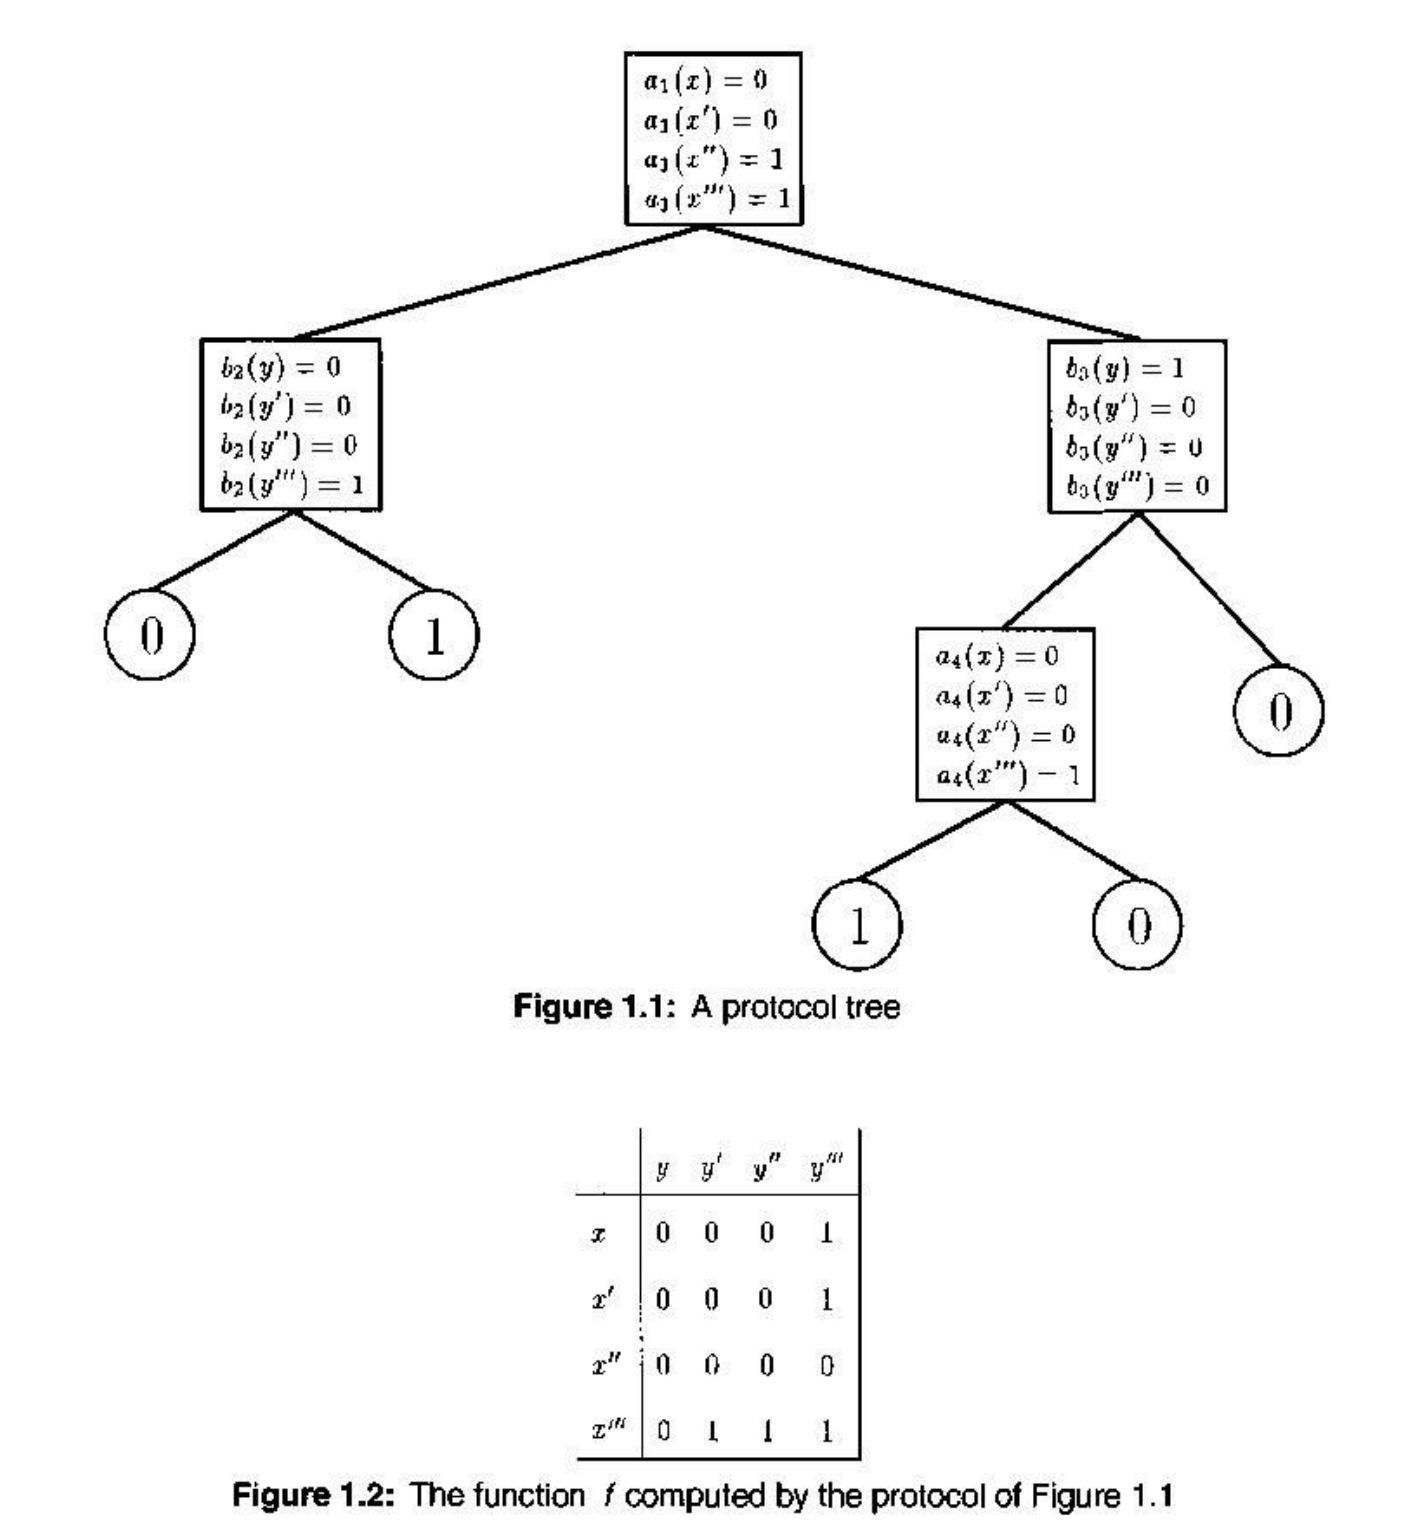
\includegraphics[width=0.5\textwidth]{protocol_tree.png}
  \caption{Protocol tree\cite{kushilevitz1997communication}}
  \label{proto_tree}
\end{figure}

By using the minimum number of square partitions $M_f$ of the function $f(x,y)$, we can derive a lower bound on the communication complexity:

\[
H(T)\ge \log_2 M_f.
\]


\begin{thm}[\cite{cr12}\cite{vidick2012concentration}\cite{sherstov2012communication}]
\label{ghd_lower_bound}
    Any randomized protocol solving problem \ref{ghd} with probability $2/3$ needs at least $\Omega(n)$ bits of communication.
\end{thm}

\pfsk{\ref{ghd_lower_bound}}{
The original proof is in \cite{cr12} and \cite{vidick2012concentration} make a simpler one. Here we use proof in \cite{sherstov2012communication}, which is simplist among them.

First, use \textbf{Yao's principle}(theorem \ref{yaoprin}) to reduce the randomness of algorithm to randomness of a distribution $\mu$ of input $(x,y)$. Formally, consider all those deterministic protocol tree $T(x,y)$ such that $\mb P_{(x,y)\sim\mu}[T(x,y)\neq f(x,y)]\le\epsilon$. Denote the minimum complexity(tree height) of such deterministic $T$ by $R_{\mu,\epsilon}(f)$, and denote minimum expectation complexity of random tree with error $\epsilon$ by $C_\epsilon(f)$, we have $C_\epsilon(f)\gtrsim R_{\mu,\epsilon}(f)$. See \cite{yao83} lemma 2 in sect. 3.3 for details.

Then, it suffices to find a hard distribution $\mu$ of $(x,y)$ and lower bound of $R_{\mu,\epsilon}(f)$.
This is done by a trick called \textbf{$\epsilon$-corruption bound}:
\begin{lem}[Yao's corruption bound\cite{sherstov2012communication}]
If $\exists \varepsilon, \delta \in(0,1)$ such that $\mu$ satisfies
$$\mu\left(R \cap f^{-1}(+1)\right)>\varepsilon \mu\left(R \cap f^{-1}(-1)\right)$$
for every rectangle $R \subseteq X \times Y$ with $\mu(R)>\delta$, 
 then $R_{\mu,\xi}(f)\ge\log_2\bbr{\frac{1}{\delta}\left(\mu\left(f^{-1}(-1)\right)-\frac{\xi}{\varepsilon}\right)}$ for small $\xi>0$.
\end{lem}
\noindent Intuitively, corruption guarantee the size of error area in each rectangle is not so small. Therefore, when total error is a given constant, we can lower bound the number of rectangle partition and thus lower bound the tree height. See \cite{yao83} lemma 3 in sect. 3.3 for originality and details. Usually, people try to directly prove corruption bound for uniformly distribution.

Finally, in our setting, the Gap-Hamming distance problem($GHD_n$) is further reduce to Gap-orthogonality problem($ORT_n$) with $R_{1/3}(GHD_n)=\Omega(R_{1/3}(ORT_n))$, where $f(x,y)=(-1)\mf 1_{|\langle x,y \rangle|\le\sqrt{n}}+(+1)\mf 1_{|\langle x,y \rangle|\ge2\sqrt{n}}$. 
Note that $f^{-1}(+1)=\{(x,y)||\langle x,y \rangle|\ge2\sqrt{n}\}$, thus the corruption bound intuitively(not so rigorously) means for rectangle $R$ with large probability, we have
\begin{equation}
    \label{anti_concen_ghd}
    \exists c,C>0,~~\mb P_{(x,y)\sim Unif[R]}[|\langle x,y \rangle|>C]\ge c,
\end{equation}
which is essentially a \textbf{anti-concentration analysis}. Choosing uniform distribution is enough, it is proved by \textbf{probabilistic method} with Talagrand's inequalities(corollary \ref{tal_ineq_proj}) and a interesting combinatorial accounting trick:
\begin{lem}[Corruption bound\cite{sherstov2012communication}]
\label{cor_bound}
Let $\mu$ be uniform distribution on $\{\pm1\}^n\times\{\pm1\}^n$ and $R=A\times B$ be a rectangle such that $\mu(R\cap f^{-1}(+1))\le \epsilon\mu(R)$ then $\mu(R)=e^{-\Omega(n)}.$ is small. In other word, if $\mu(R)$ is large, we have corruption bound.
\end{lem}
\pfskm{lemma}{\ref{cor_bound}}{
The anti-concentration inequality is reduced to that, by corollary \ref{tal_ineq_proj} we can find a set $I$ of near-orthogonal vectors of $x\in A$ in rectangle $R=A\times B$ with large probability, and then by some linear algebra and Hoffman-Wielandt inequality, for most of $y\in B$, there must exists a $x'\in I$ such that $|\langle x',y\rangle|$ is large. 
}
\noindent Use the lemma, we compute $C_{1/3}(GHD_n)=\Omega(R_{1/3}(ORT_n))=\Omega(n)$.
}

\begin{rmk}
For general communication problem, the analysis of average-case complexity usually follows the roadmap above:
\begin{enumerate}
    \item Use Yao's principle to reduce the problem with randomized algorithm into a randomized input with deterministic algorithm.
    \item Find the math structures of complexity in setting of deterministic algorithm(In communication problem, it's height of a binary tree whose leaf nodes are rectangle partition).
    \item Abstract these structures into pure math language, and then use fundamental math tool to work it out(In this communication function $f=GHD_n$, the structure is an anti-concentration analysis and tools are some probabilistic methods).
\end{enumerate}
\end{rmk}

\begin{rmk}
Another proof\cite{vidick2012concentration} use a different description of the anti-concentration(theorem \ref{large_overlap}) in corruption bound \eqref{anti_concen_ghd}, where they consider general vectors $x,y\in\R^n$($\mc X,\mc Y, R$ may be continuous).
\end{rmk}

%---------------------------------------------------
\subsection{Spiked wishart matrix testing}
\begin{prob}[Spiked wishart matrix\cite{mmmw21}\cite{pwbm18}]
\label{spiked_wishart}
Let $n=1/\epsilon$ and let $z\in\R^n$ be a uniformly random unit vector. Let $N\in\R^{n\times m}$ be $m$ $i.i.d$ Gaussian vector drawn from an $n$-dimensional $\mc N(0,C)$, where $C=I$ or $I-zz^T$. Use $N$ to identify $C$.
\end{prob}

\begin{thm}[\cite{mmmw21}]
\label{spiked_whishart_lower_bound}
To solve problem \ref{spiked_wishart} with probability at least $2/3$, we need at least $m=\Omega\bbr{\frac{1}{\epsilon}}$.
\end{thm}
\pfsk{\ref{spiked_whishart_lower_bound}}{First, let $P$ denote the distribution of $N$ under null hypothesis $C=I$, and $Q$ denote the distribution of $N$ under alternative hypothesis $C=I-zz^T$. Any testing statistics $\phi$ outputs $1$ for $Q$ and $0$ for $P$. It suffices to bound the total variation distance $d_{TV}(P,Q)$, since its control the summation of Type-1 and Type-2 errors
\begin{align*}
    \min_\phi\bbwr{P(\phi=1)+Q(\phi=0)}=1-d_{TV}(P,Q).
\end{align*}

Then, by Pinsker's inequality, we have $d_{TV}(Q,P)\le\sqrt{\frac{1}{2}D_{KL}(Q||P)}\le\sqrt{\frac{1}{2}D_{\chi^2}(Q||P)}.$
Therefore it suffices to upper bound $D_{\chi^2}(Q||P)=\int_{N}\bbr{\frac{Q(N)}{P(N)}}^2P(N)dN - 1$. By theorem \ref{spiked_gaussian_chi_dist} with $\beta=-1$ and spiked prior $z$, we have
\begin{align*}
    D_{\chi^2}(Q||P) = \mb E_{v,v'}\bbfr{(1-\langle v,v' \rangle^2)^{-m/2}}-1,
\end{align*}
where $v,v\stackrel{\mathrm{dist}}{=}z$ are uniformly random unit vectors. Therefore, by classical results of random unit vectors, $p.d.f.$ of $x:=\langle v, v'\rangle$ is $p(x)=\frac{\Gamma(n-1)}{2\Gamma((n-1)/2)^2}\bbr{\frac{1-x^2}{4}}^{(n-1)/2-1}$.

Finally, direct calculation yields, if $m=O\bbr{1/\epsilon}$, $\mb E_{v,v'}\bbfr{(1-\langle v,v' \rangle^2)^{-m/2}}<6/5$ and thus $d_{TV}(Q,P)<1/3$. Therefore, one of Type-1 and Type-2 errors must be larger than $1/3$.
}

\begin{prob}[\cite{jpwz21}]
    \label{hard_psd_testing}
    Given $\delta\in(0,1/2)$, set $n=\log(1/\delta)$. Independently take $g\sim\mc N(0,I_n)$ and $G\in\R^{n\times n}$ with $i.i.d.$ $\mc N(0,1)$ entries. Let $W=G+G^T$. Consider two distributions:
    \begin{itemize}
        \item Distribution $P$: $C\log^{3/2}(1/\delta)\cdot\frac{1}{\|g\|_2^2}gg^T + W + 6\sqrt{\log(1/\delta)}I_n$ for some fixed constant $C>0$.
        \item Distribution $Q$: $W + 6\sqrt{\log(1/\delta)}I_n$.
    \end{itemize}
    Use \textbf{non-adaptive} queries $q_1,...q_m$ and oracles $Aq_1,...,Aq_m$ to distinguish $P$ and $Q$. In other word, take a matrix $Q\in\R^{n\times m}$ as query and $AQ$ as oracle.
\end{prob}
\begin{thm}[\cite{jpwz21}]
    \label{hard_psd_testing_bound}
    Any randomized algorithm solving problem \ref{hard_psd_testing} with probability $1-\delta$ need at least $m=\Omega\bbr{\frac{\log(1/\delta)}{\log\log(1/\delta)}}$ queries. 
\end{thm}
\pfsk{\ref{hard_psd_testing_bound}}{
Similar to the proof of theorem \ref{spiked_whishart_lower_bound}, it is naturally to consider bounding the total variation $d_{TV}(P,Q)$, and by rotational invariance we WLOG assume $Q=E_m$, the first $m$ standard basis vectors. 

First, denote by $P',Q'$ the distribution of $BQ$($B\sim P$ or $Q$ respectively). Let $L_{P'},L_{Q'}\in\R^{l}$ be vectorization of matrices from $P',Q'$(remove the redundant variable, since $B$ is symmetric), where $l=n+(n-1)+\cdots (n-m+1)$. Observe that conditioned on a realization $g$ we have
\begin{align*}
    d_{KL}(P',Q'|g)&\le d_{KL}(L_{P'},L_{Q'}|g)
    \le \|\mb EL_{P'} - \mb EL_{Q'}\|_2^2=\sum_{i=1}^m\left\|C\log^{3/2}(1/\delta)\frac{gg^T}{\|g\|_2^2}e_i\right\|_2^2=C^2\log^{3}(1/\delta)\frac{\|g^T Q\|_2^2}{\|g\|_2^2}.
\end{align*}
The first inequality use data processing inequality(theorem \ref{data_process}) and the second inequality uses theorem \ref{gauss_kl}.

Then, find a typical event $\mc E$ with positive probability. We take $\mc E=\bbwr{\frac{\|g^T Q\|_2^2}{\|g\|_2^2}\le\frac{1}{50C^2n^3}}$ and show that $\mb P(\mc E)\ge 10\delta$ if we only take $m=O\bbr{\frac{\log(1/\delta)}{\log\log(1/\delta)}}$ queries. Indeed, assume $m\le n/2$
$$
\mb P(\mc E)\ge \mb P(\|g\|_2^2\ge n/2|\|g^T Q\|_2^2\ge 1/(100C^2n^2))\cdot\mb P(\|g^T Q\|_2^2\ge 1/(100C^2n^2))
= \Omega(1)\cdot\Omega((\frac{1}{n\sqrt{m}})^m)=\Omega(e^{-\frac{m}{2}\log(n^2m)}).
$$
Therefore, when $m=O\bbr{\frac{\log(1/\delta)}{\log\log(1/\delta)}}$, $\mb P(\mc E)\ge 10\delta$.

Finally, conditioned realization $g\in\mc E$, we have the total variation $d_{TV}(P',Q'|g)\le\sqrt{d_{TV}(P',Q'|g)/2}\le 1/3$ by Pinsker's inequality. This means $\mb P[\text{the algorithms make mistake}|g]\ge 1/3$ under $P'$ or $Q'$. Since $\mb P(\mc E)\ge 10\delta$, we have $\mb P[\text{the algorithms make mistake}]\ge \delta$ under $P$ or $Q$ if we only take $m=O\bbr{\frac{\log(1/\delta)}{\log\log(1/\delta)}}$ queries.
}
\xb{consider directly bound $d_{TV}(P,Q)\le 1-2\delta$ instead?}
%---------------------------------------------------
%---------------------------------------------------
%---------------------------------------------------
\chapter{Math Foundation}
Basic math tools.

%---------------------------------------------------
%---------------------------------------------------
\section{Key elements}
\subsection{Yao's principle}
When we analyze complexity of average-case problem with randomized algorithm, we can analyze a problem with randomized input and deterministic algorithm instead.
\begin{thm}[Yao's minimax principle\cite{yao_prin}]
 \label{yaoprin}
Given a problem $\mc P$, let $\mc A$ be the set of all deterministic algorithms to solve $\mc P$ and $\mc X$ be the set of all instances of $\mc P$.
Let $c(a,x)$ be the cost of algorithm $a\in\mc A$ solving instance $x\in\mc X$. For any distribution $p$ over $\mc A$ and any distribution $q$ over input space $\mc X$, consider randomized algorithm $A\sim p$ and random instance $X\sim q$. Then, we have
$$
\max _{x \in \mathcal{X}} \mathbf{E}[c(A, x)] \geq \min _{a \in \mathcal{A}} \mathbf{E}[c(a, X)]
$$
\end{thm}
That is, the worst-case expected cost of the randomized algorithm is at least the expected cost of the best deterministic algorithm against input distribution $q$.
\pf{\ref{yaoprin}}{
Let $C=\max _{x \in \mathcal{X}} \mathbf{E}[c(A, x)]$ and $D=\min _{a \in \mathcal{A}} \mathbf{E}[c(a, X)]$. We have
$$
\begin{aligned}
C & =\sum_x q_x C  \geq \sum_x q_x \mathbf{E}[c(A, x)]  =\sum_x q_x \sum_a p_a c(a, x)=\sum_a p_a \sum_x q_x c(a, x)  =\sum_a p_a \mathbf{E}[c(a, X)]  \geq \sum_a p_a D=D
\end{aligned}
$$
}


%---------------------------------------------------
%---------------------------------------------------
\section{Concentration inequalities}


%---------------------------------------------------
\subsection{Overlap of a vector on a large set}
If two subsets of $\R^n$ are "large", then the "overlap" of them is large. Here, "large" means the subsets have large meassure under Gaussian measure, and "overlap" means: For any non-empty $A,B\subseteq \R^n$. Denote by $\gamma_{|A\times B}$ the probability measure corresponding to the normalized restriction of $\mc N(0,I_n)\times \mc N(0,I_n)$ to $A\times B$ and let
\[
v(A,B):=\mb E_{(x,y)\sim\gamma_{|A\times B}}[|\langle x,y \rangle|^2].
\]
Formally, we have
\begin{thm}[\cite{vidick2012concentration}]
\label{large_overlap}
For any $\eta>0$, there exists ${ }^1$ a $\delta>0$ such that for all large enough $n$, if $A, B$ both have measure $\gamma(A), \gamma(B) \geq e^{-\delta n}$ then
$$
v(A, B) \geq(1-\eta) v\left(\mathbb{R}^n, \mathbb{R}^n\right)=(1-\eta) n
$$
\end{thm}
It's continuous version of \eqref{anti_concen_ghd}, which is more general to yield corruption bound for communication problem with continuous domain $\mc X,\mc Y$ and rectangle $R$.
%---------------------------------------------------
\subsection{Hutchinson's trace estimator}
A simple estimator of trace of matrix by monte carlo method and we use only matrix-vector product oracle.
\begin{defn}[Hutchinson's Estimator]
\label{hutchinson_est}
Given a matrix $A\in\R^{d\times d}$. We estimate $tr(A)$ by
\[
H_m(A) = \frac{1}{m}\sum_{i=1}^m g_i^T A g_i = \frac{1}{m}tr(G^T A G),
\]
where $G=[g_1,...,g_m]\in\R^{d\times m}$ is a Gaussian matrix with $i.i.d.$ $\mc N(0,1)$ entries.
\end{defn}

\begin{thm}[Hutchinson analysis\cite{mmmw21}]
\label{hutchinson_bound}
Let $A \in \mathbb{R}^{d \times d}, \delta \in(0,1 / 2], \ell \in \mathbb{N}$. Let $\mathrm{H}_{\ell}(A)$ be the $\ell$-query Hutchinson estimator defined in (1), implemented with mean 0, i.i.d. sub-Gaussian random variables with constant sub-Gaussian parameter. For fixed constants $c, C$, if $\ell>c \log (1 / \delta)$, then with probability $\geq 1-\delta$,
$$
\left|\mathrm{H}_{\ell}(A)-\operatorname{tr}(A)\right| \leq C \sqrt{\frac{\log (1 / \delta)}{\ell}}\|A\|_F .
$$
So, if $\ell=O\left(\frac{\log (1 / \delta)}{\varepsilon^2}\right)$ then, with probability $\geq 1-\delta,\left|\mathrm{H}_{\ell}(A)-\operatorname{tr}(A)\right| \leq \varepsilon\|A\|_F$.
\end{thm}
\pfsk{\ref{hutchinson_bound}}{
First, vectorize gaussian matrix $G$ to $\bar{g}\in\R^{dl}$ and let $\bar{A}=diag\{A,A,...,A\}\in\R^{dl\times dl}$.

Then, $H_l(A)=\bar{g}^T\bar{A}\bar{g}/l$ and use Hanson-Wright inequality\cite{hdp}.
}

%---------------------------------------------------
\subsection{Talagrand's inequality}
\begin{thm}[Talagrand\cite{sherstov2012communication}]
\label{tal_ineq}
For a fixed convex set $S \subseteq \mathbb{R}^n$ and a random $x \in\{-1,+1\}^n$,
$$
\mathbb{P}[x \in S] \mathbb{P}[\rho(x, S)>t] \leq \mathrm{e}^{-t^2 / 16},
$$
where $\rho(x, S)=\inf _{y \in S}\|x-y\|$.
\end{thm}
Intuitively, it means measure concentration around convex hull of large subset $S\subseteq\{\pm 1\}^n$, where the measure means counting measure(or uniform distribution). It can be seen as an isoperimetric inequality in discrete structures.

The usefulness of Talagrand's inequality is led by appropriately choosing set $S$, according to property we interest. Here are some useful corollaries.
\begin{cor}[\cite{sherstov2012communication}]
\label{tal_ineq_proj}
For every linear subspace $V \subseteq \mathbb{R}^n$ and every $t>0$, one has
$$
\underset{x \in\{-1,+1\}^n}{\mb{P}}\left[\left|\left\|\operatorname{proj}_V x\right\|-\sqrt{\operatorname{dim} V}\right|>t\right]<4 \mathrm{e}^{-c t^2},
$$
where $c>0$ is an absolute constant.
\end{cor}
\pf{\ref{tal_ineq_proj}}{ First, note that it suffices to prove
$$
\mathbf{P}[|\rho(x, V)-\sqrt{n-\operatorname{dim} V}|>t] \leq 4 \mathrm{e}^{-\Omega\left(t^2\right)}
$$
and $n-\operatorname{dim} V= tr(\mb E[x^T(I-P_V)x]) =\mb E[\rho(x,V)^2]$, where $P_v$ is orthogonal projection on $V$.
 Therefore, take $S=\{v\in\R^n:\rho(v,V)\le a\}$, then by Talagrand's inequality we have
\[
\mathbb{P}[\rho(x, V) \leq a] \mathbb{P}[\rho(x, V)>a+t] \le \mathbb{P}[\rho(x, V) \leq a] \mathbb{P}[\rho(x, S)>t]  \leq \mathrm{e}^{-t^2 / 16}.
\]
Then, take $a=median(\rho(x,V)):=m$, we have
$$
\begin{aligned}
& \mathbb{P}[\rho(x, V)>m+t] \leq 2 \mathrm{e}^{-t^2 / 16}, \\
& \mathbb{P}[\rho(x, V) \leq m-t] \leq 2 \mathrm{e}^{-t^2 / 16}.
\end{aligned}
$$
Finally, the result follows $m=\sqrt{\mb E[\rho(x,V)^2]}+O(1)$. See \cite{tao09web} for details.
}

%---------------------------------------------------
%---------------------------------------------------
\section{Statistical distance}
\begin{thm}[\cite{pwbm18} proposition 5.11]
\label{spiked_gaussian_chi_dist}
For any $|\beta|<1$, there exists $\delta>0$ such that the following holds. Let $\mc X=\{\mc X_n\}$ be a family of prior distribution of spiked vectors $x$ with $1-\delta\le\|x\|\le 1+\delta$. Let $Q_n$ be joint distribution of $N$ $i.i.d$ samples from $\mc N(0,I_n+\beta xx^T)$ and $P_n$ be joint distribution of $N$ $i.i.d$ samples from $\mc N(0,I_n)$. Then we have
\[
\mb E_{P_n}\bbfr{\bbr{\frac{dQ_n}{dP_n}}^2} = \mb E_{x,x'\sim\mc X_n}\bbfr{(1-\beta^2\langle x,x' \rangle^2)^{-N/2}}.
\]
\end{thm}
\pf{\ref{spiked_gaussian_chi_dist}}{
First, expand LHS directly, we have $ \underset{P_n}{\mathbb{E}}\left[\left(\frac{\mathrm{d} Q_n}{\mathrm{~d} P_n}\right)^2\right]=\underset{Q_n}{\mathbb{E}}\left[\frac{\mathrm{d} Q_n}{\mathrm{~d} P_n}\right]$
$$
\begin{aligned}
& \frac{\mathrm{d} Q_n}{\mathrm{~d} P_n}\left(y_1, \ldots, y_N\right)=\underset{x^{\prime} \sim \mathcal{X}}{\mathbb{E}}\left[\prod_{i=1}^n \frac{\exp \left(-\frac{1}{2} y_i^{\top}\left(I+\beta x^{\prime} x^{\prime \top}\right)^{-1} y_i\right)}{\sqrt{\operatorname{det}\left(I+\beta x^{\prime} x^{\prime \top}\right)} \exp \left(-\frac{1}{2} y_i^{\top} y_i\right)}\right] \\
& =\underset{x^{\prime}}{\mathbb{E}}\left[\operatorname{det}\left(I+\beta x^{\prime} x^{\prime \top}\right)^{-N / 2} \prod_{i=1}^N \exp \left(-\frac{1}{2} y_i^{\top}\left(\left(I+\beta x^{\prime} x^{\prime \top}\right)^{-1}-I\right) y_i\right)\right] .
\end{aligned}
$$
Then, simplify it by  Sherman–Morrison formula, we have $\left(I+\beta x^{\prime} x^{\prime \top}\right)^{-1}-I=\frac{-\beta}{1+\beta\left\|x^{\prime}\right\|^2} x^{\prime} x^{\prime \top}$, and then
$$
=\underset{x^{\prime}}{\mathbb{E}}\left[\left(1+\beta\left\|x^{\prime}\right\|^2\right)^{-N / 2} \prod_{i=1}^N \exp \left(\frac{1}{2} \frac{\beta}{1+\beta\left\|x^{\prime}\right\|^2}\left\langle y_i, x^{\prime}\right\rangle^2\right)\right] .
$$
Finally, passing to the second moment, we compute
$$
\begin{aligned}
& \underset{P_n}{\mathbb{E}}\left[\left(\frac{\mathrm{d} Q_n}{\mathrm{~d} P_n}\right)^2\right]=\underset{x, x^{\prime}}{\mathbb{E}}\left[\left(1+\beta\left\|x^{\prime}\right\|^2\right)^{-N / 2} \prod_{i=1}^N \underset{y_i \sim \mathcal{N}\left(0, I+\beta x x^{\top}\right)}{\mathbb{E}} \exp \left(\frac{1}{2} \frac{\beta}{1+\beta\left\|x^{\prime}\right\|^2}\left\langle y_i, x^{\prime}\right\rangle^2\right)\right]\\
& =\underset{x, x^{\prime}}{\mathbb{E}}\left[\left(1+\beta\left\|x^{\prime}\right\|^2\right)^{-N / 2} \prod_{i=1}^N\left(1-\frac{\beta}{1+\beta\left\|x^{\prime}\right\|^2}\left(\left\|x^{\prime}\right\|^2+\beta\left\langle x, x^{\prime}\right\rangle^2\right)\right)^{-1 / 2}\right] \\
& =\underset{x, x^{\prime}}{\mathbb{E}}\left[\left(1-\beta^2\left\langle x, x^{\prime}\right\rangle^2\right)^{-N / 2}\right]
\end{aligned}
$$
Note that, the condition about $\delta$ is because here the MGF step requires
$
\frac{\beta}{1+\beta\left\|x^{\prime}\right\|^2}\left(\left\|x^{\prime}\right\|^2+\beta\left\langle x, x^{\prime}\right\rangle^2\right)<1
$.
}

\begin{thm}[\cite{jpwz21}]
\label{gauss_kl}
For distribution $P=\mc N_k(\mu_1,\Sigma_1)$ and $Q=\mc N_k(\mu_2,\Sigma_2)$, we have
\[
d_{KL}(P,Q)=\frac{1}{2}\bbwr{
(\mu_2-\mu_1)^T\Sigma_2^{-1}(\mu_2-\mu_1)
+ tr(\Sigma_2^{-1}\Sigma_1) - \log\frac{det(\Sigma_1)}{det(\Sigma_2)-k}
}.
\]
\end{thm}

\begin{thm}[Data processing inequality\cite{jpwz21}]
\label{data_process}
For random variable $X,Y$ and any function $f$, we have
\[
d_{KL}(f(X),f(Y))\le d_{KL}(X,Y).
\]
\end{thm}
%---------------------------------------------------
%---------------------------------------------------
\section{Random matrices}
In this section, we denote the distribution of random matrices $G\in\R^{n\times n}$ with $i.i.d.$ $\mc N(0,1)$ entries by $\mc N(n)$.
\begin{thm}[Remaining randomness\cite{simchowitz2020tight}\cite{jpwz21}]
\label{block_conditional} 
Let $G\sim\mc N(n)$. Let $W=(G+G^T)/2$. For any sequence of vector queries $v_1,...,v_T$, along with oracles $w_i=Wv_i$. Then, conditioned on these observations, there exists a rotation matrix $U$, independent of $w_i$, such that
\[
UWU^T=\begin{bmatrix}
    Y_1 & Y_2^T \\
    Y_2 & \widetilde{W}
\end{bmatrix},
\]
where $Y_1,Y_2$ are deterministic and $\widetilde{W}=(\widetilde{G}+\widetilde{G}^T)/2$, where $\widetilde{G}\sim\mc N(n-T)$.
\end{thm}
\pfsk{\ref{block_conditional}}{

}

\begin{thm}[concentration of the largest singular value\cite{jpwz21}]
\label{rmt_smax_concen}
Let $G\sim\mc N(n)$. Then, for any $t\ge 0$ we have
\[
\mb P[s_{max}(G)\le 2\sqrt{n}+t]\ge 1-2e^{-t^2/2}.
\]
\end{thm}
\pfsk{\ref{rmt_smax_concen}}{
    
}

%---------------------------------------------------
%---------------------------------------------------
%---------------------------------------------------



%---------------------------------------------------
% \printbibliography
\bibliographystyle{apalike}
\bibliography{cite.bib}
\end{document}
